\documentclass[../../main.tex]{subfiles}
\begin{document}

In general, there are two approaches to evolve creatures, what we will call \textit{Instance Evolution}, and \textit{Continuous Evolution}. Instance evolution takes place on a single creature and progress occurs in discrete iterations. By contrast, Continuous Evolution simulates multiple creatures simultaneously resulting in a more realistic continuous evolution. The former has a more straightforward implementation (including parallelization) and is expected to improve faster. The latter however greatly reduces computational cost for large scale simulations. This has not yet been implemented, but may be when creatures can detect and react to other creatures. The following will only discuss instance evolution.

There are several components that work together to allow for high configurability and expandability. The simplest component is the \textbf{gene}. These encoded the properties of a component of a \textbf{creature}. The set of these are packaged into a \textbf{genome}, which in turn can be decoded into a physical entity according to a \textbf{body}'s interpretation of the genes, resulting in a \textbf{creature}. This is sufficient to create an entity but to simulate and evolve it, it requires \textcolor{red}{both a \textbf{fitness} metric to strive for and [This is a poor design and should be directly connected to the Evolution Algorithm]} an \textbf{environment} that it may interact with, in what is referred to as a \textbf{scenario}. Multiple scenarios, contained in a \textbf{population} are required to be simulated for the \textbf{evolution algorithm} to be used effectively. Finally, the \textbf{user} may interact / view aspects entities in the population through the \textbf{Viewer} class. An overview of these components can be found in Fig.~\ref{fig:overview}. They will be individually discussed in the following sections.
\begin{figure}[H]
	\centering
	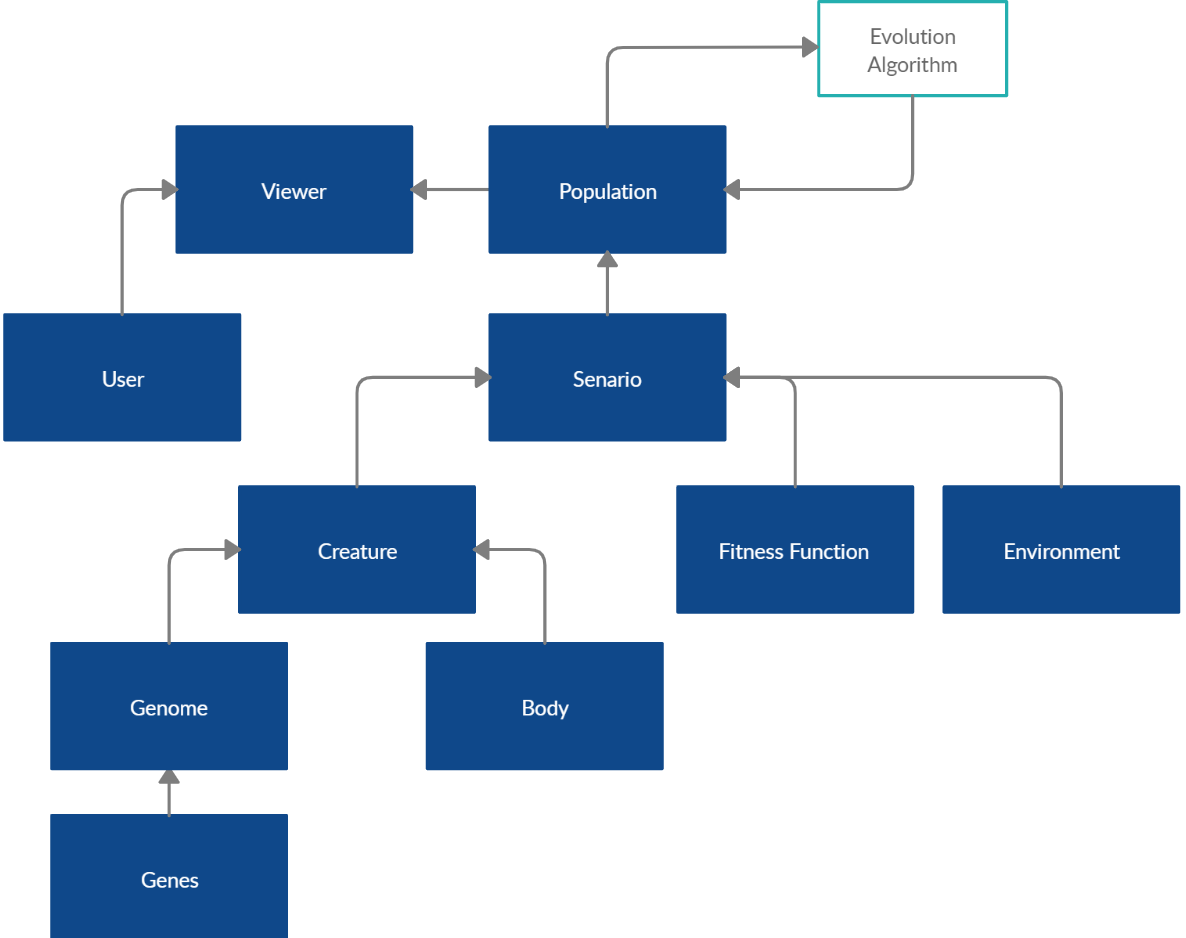
\includegraphics[width=\textwidth]{img/hierarchy.png}
	\caption{The machinery that allows the user to view the evolution of a set of genes expressed by a body in a given environment according to a given fitness function. Opaque boxes correspond to classes, while clear boxes correspond to procedures.}
	\label{fig:overview}
\end{figure}

\section{Genetics}
	\subsection{Genes}
		A gene is very simple as it only contains a set of attributes representing the properties of a component of a creature. They may be read to/from a string. Every gene has a unique (single-character) symbol associated with it, so that the string representation is uniquely identified.
		Several genes are already implemented:
		\begin{center}
			\begin{minipage}{13cm}
			\dirtree{%
				.1 Gene.
					.2 NodeGene \DTcomment{\verb|Vec3 position, double mass, double friction}.
					.2 BoneGene \DTcomment{\verb|int a, int b}.
						.3 MuscleGene \DTcomment{\verb|int a, int b, double speed}.
					.2 CubeGene \DTcomment{\verb|Vec3 position, double mass}.
					.2 AxonGene \DTcomment{\verb|int a, int b, int layer, double weight}.
			}%|
			\end{minipage}
		\end{center}
	\subsection{Genome}
		A genome is a collection of genes. It can be written to/from a string. It can also be mutated, resulting in potentially altered genes. The usability of this is relatively low and currently is manually controlled.

	\subsection{Open-Questions}
		\begin{itemize}
			\item The single-character notation may quickly cause expressiveness to degrade as name collisions are avoided. A string symbol would avoid this.

			\item How should mutations for different creatures be managed? Most likely each \verb|body| should be in control of this.
		\end{itemize}

\section{Physical}
	\subsection{Body}
	\subsection{Creature}
	\subsection{Environment}
	\subsection{Scenario}

\section{Algorithm}
	\subsection{Population}

\section{Viewer}

\section{Special Details}
	The evolution algorithm is multi-threaded.

\end{document}